\section{Video-LDM}
\label{sec:videoldm}

\begin{figure}
    \centering
    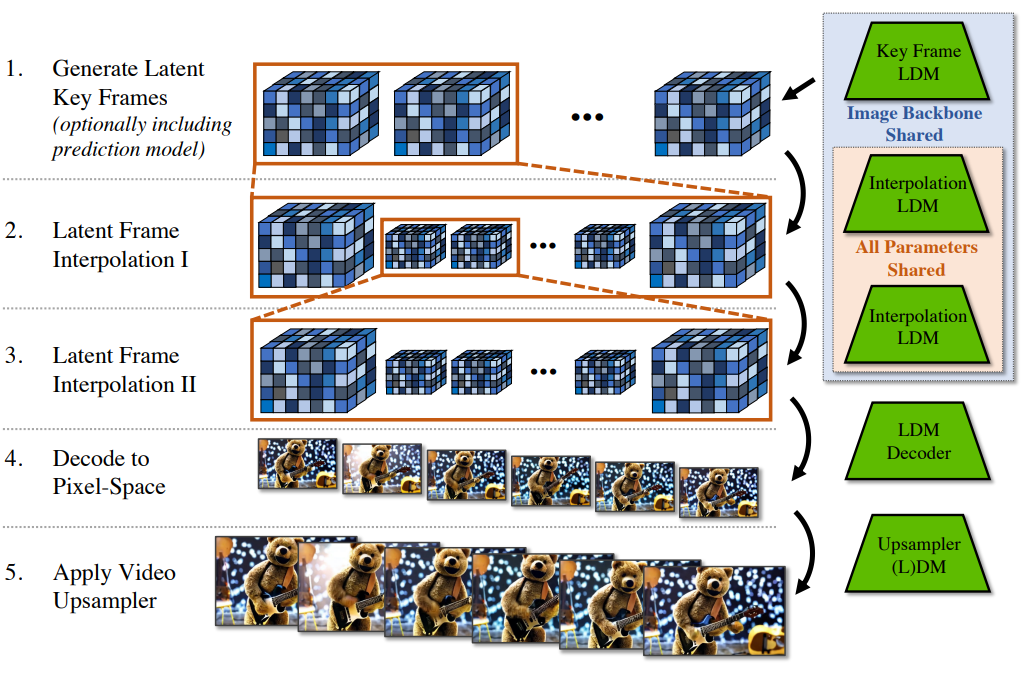
\includegraphics[width=0.8\textwidth]{images/video_ldm/stack.png}
    \caption{Video-LDM stack. (1) The network generates keyframes latents. (2) Between each two keyframes, the network learns to interpolate between (keyframe filling). (3) Between each two frames in the frame filling, they act as new keyframes and the process repeats once more. (4) The latents are decoded to pixel space. (5) Super-resolution model is applied (optionally) to upsample the video resolution.}
\end{figure}

Video-LDM by NVIDIA (2023) \cite{video_ldm} is a text-to-video synthesis model that uses LDM (Latent Diffusion Model, more commonly called Stable Diffusion, section \ref{sec:stable_diffusion}). The main idea of Video-LDM is to first train the model as image generator; and then transform it into a video generator. Its also possible to use pre-trained LDM and then fine-tune it and convert it to a video generator. The model can output in a resolution of up to 1280x2048, which is considered very high resolution in the field of video synthesis.

First, the model is pre-trained with image only datasets; then, temporal layers are added to the LDM that learn to align images in temporally consistent manner; then the model is trained on video datasets and only the temporal layers are learned (the other layers are frozen). They demonstrated that the learned temporal layers can be combined with different image model checkpoints.

\begin{figure}
    \centering
    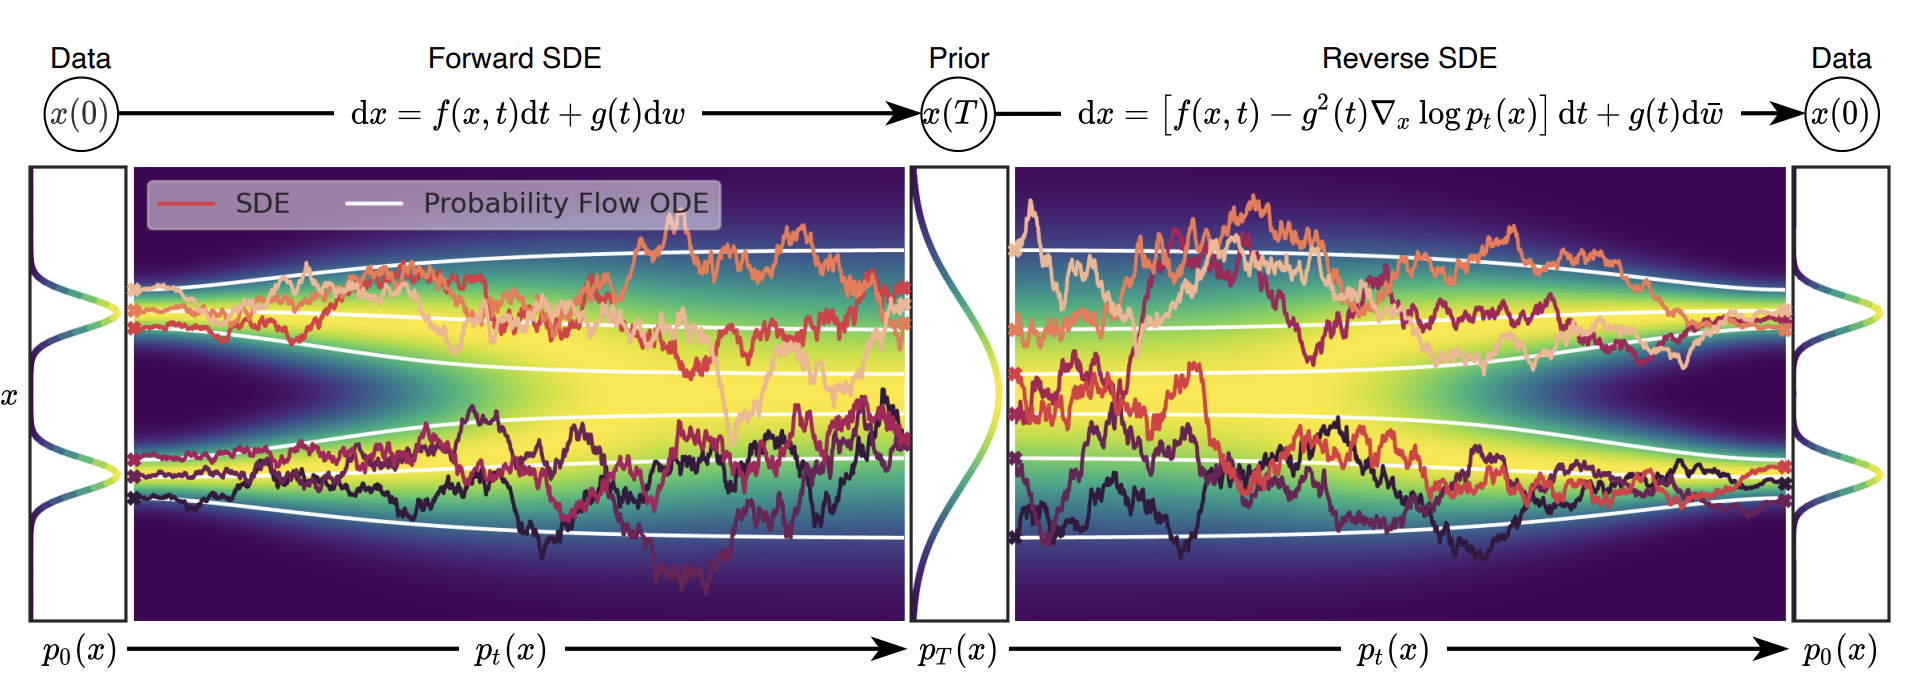
\includegraphics[width=0.8\textwidth]{images/video_ldm/ddpm_sde.png}
    \caption{Generative modeling through stochastic differential equations (SDE) \cite{song2020score}. It shows how data distribution $p(x)$ slowly transforms to prior distribution $p_T(x)$ through forward SDE (we add noise) and then reversed back to generate data with reverse SDE. The colored lines show the SDE paths which represent sample trajectories through the diffusion process. The lines converge at the prior, the noise causes data samples to become progressively less structured, transitioning from a well-defined data distribution to a more chaotic noise-like distribution. The left side shows the probability of the data, the middle shows the probability of the prior (Gaussian distribution), and the right shows we are back to the original data distribution.}
\end{figure}

\begin{figure}
    \centering
    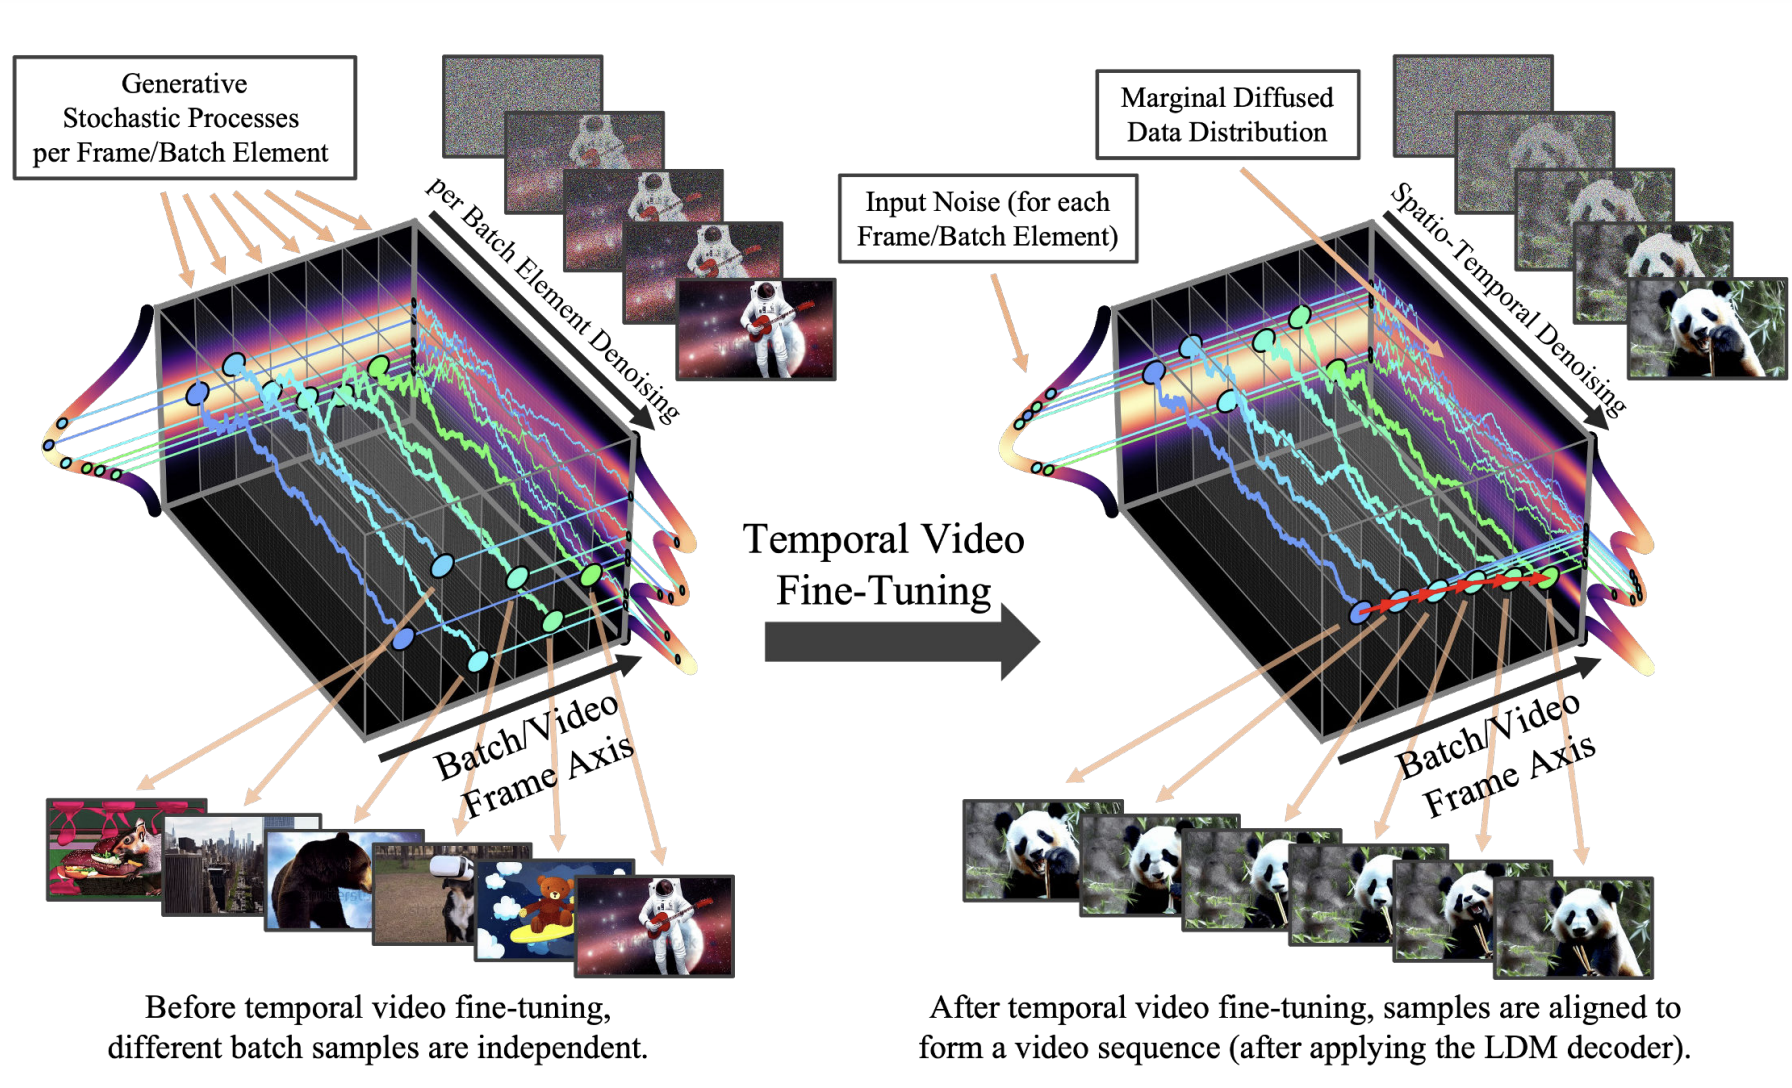
\includegraphics[width=0.8\textwidth]{images/video_ldm/image_to_video_tuning.png}
    \caption{Transforming image LDM (left) to video LDM (right) \cite{video_ldm}. \textit{Per-batch element denoising}: the stochastic denoising process of diffusion. \textit{Batch/Video Frame Axis}: on the left each image generated is not correlated to other images in the batch; on the right each generated image is correlated to the previous image, the model learns to align them and generate temporally consistent video. \textit{Batch/Video Frame Axis}: the red arrows and line shows how one image transitions to the next image, creating the video.}
    \label{fig:video_ldm_image_to_video_tuning}
\end{figure}

\subsection*{Mathematical notations}

The LDMs autoencoder compresses the high-dimensional input data $x \in \mathbb{R}^{T \times 3 \times \hat{H} \times \hat{W}}$ where $x \sim p_{\text{data}}$ is a sequence of $T$ RGB frames with height $\hat{H}$ and width $\hat{W}$ to lower-dimensional latent space $z = \mathcal{E} (x) \in \mathbb{R}^{T \times C \times H \times W}$ (where $C$ is the number of latent channels, and $H, W$ are the spatial latent dimensions) in order to improve computational needs. The model then learns to reconstruct $x$ via decoder $\mathcal{D}$: $\hat{x} = \mathcal{D} (\mathcal{E} (x)) \sim x$.

Let us denote the layers of the LDM (without temporal layers) as spatial layers $l^i_{\theta}$ where $\theta$ are the model's parameters, and $i$ is the layer index. We then denote the addition of temporal layers as $l^i_{\phi}$ to learn to align individual frames in a temporally consistent manner. We denote $f_{\theta, \phi}$ as the full model (with spatial and temporal layers).

\subsection{Architecture}

\begin{figure}
    \centering
    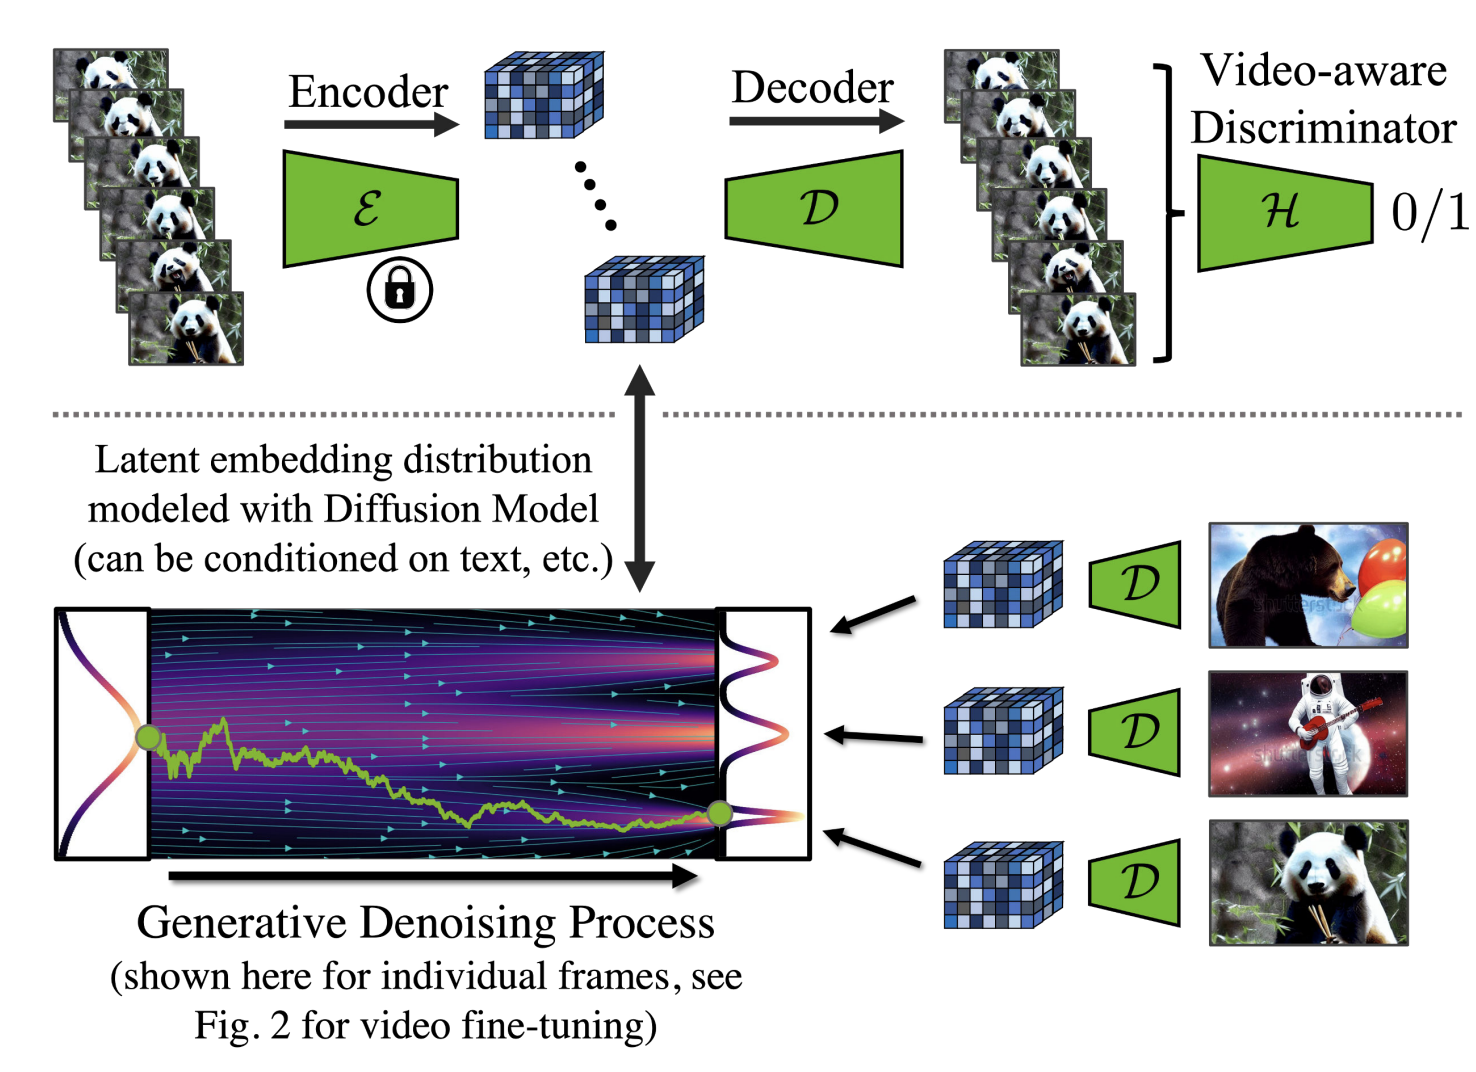
\includegraphics[width=0.6\textwidth]{images/video_ldm/enc_dec_denoise_process.png}
    \caption{Top: frozen encoder compresses video frames into 3D latents and the decoder learns to reconstruct image from the latent (like in autoencoders). The patch-based discriminator $\mathcal{H}$ is used to increase photorealism, the adversarial objective is added to the autoencoder reconstruction score like in PatchGAN (\cite{isola2017image} which tries to classify if $N \times N$ patch is real or fake). \textit{Bottom}: generative denoising process, each embedding corresponds to different image generation in the decoder $\mathcal{D}$.}
\end{figure}

\begin{figure}
    \centering
    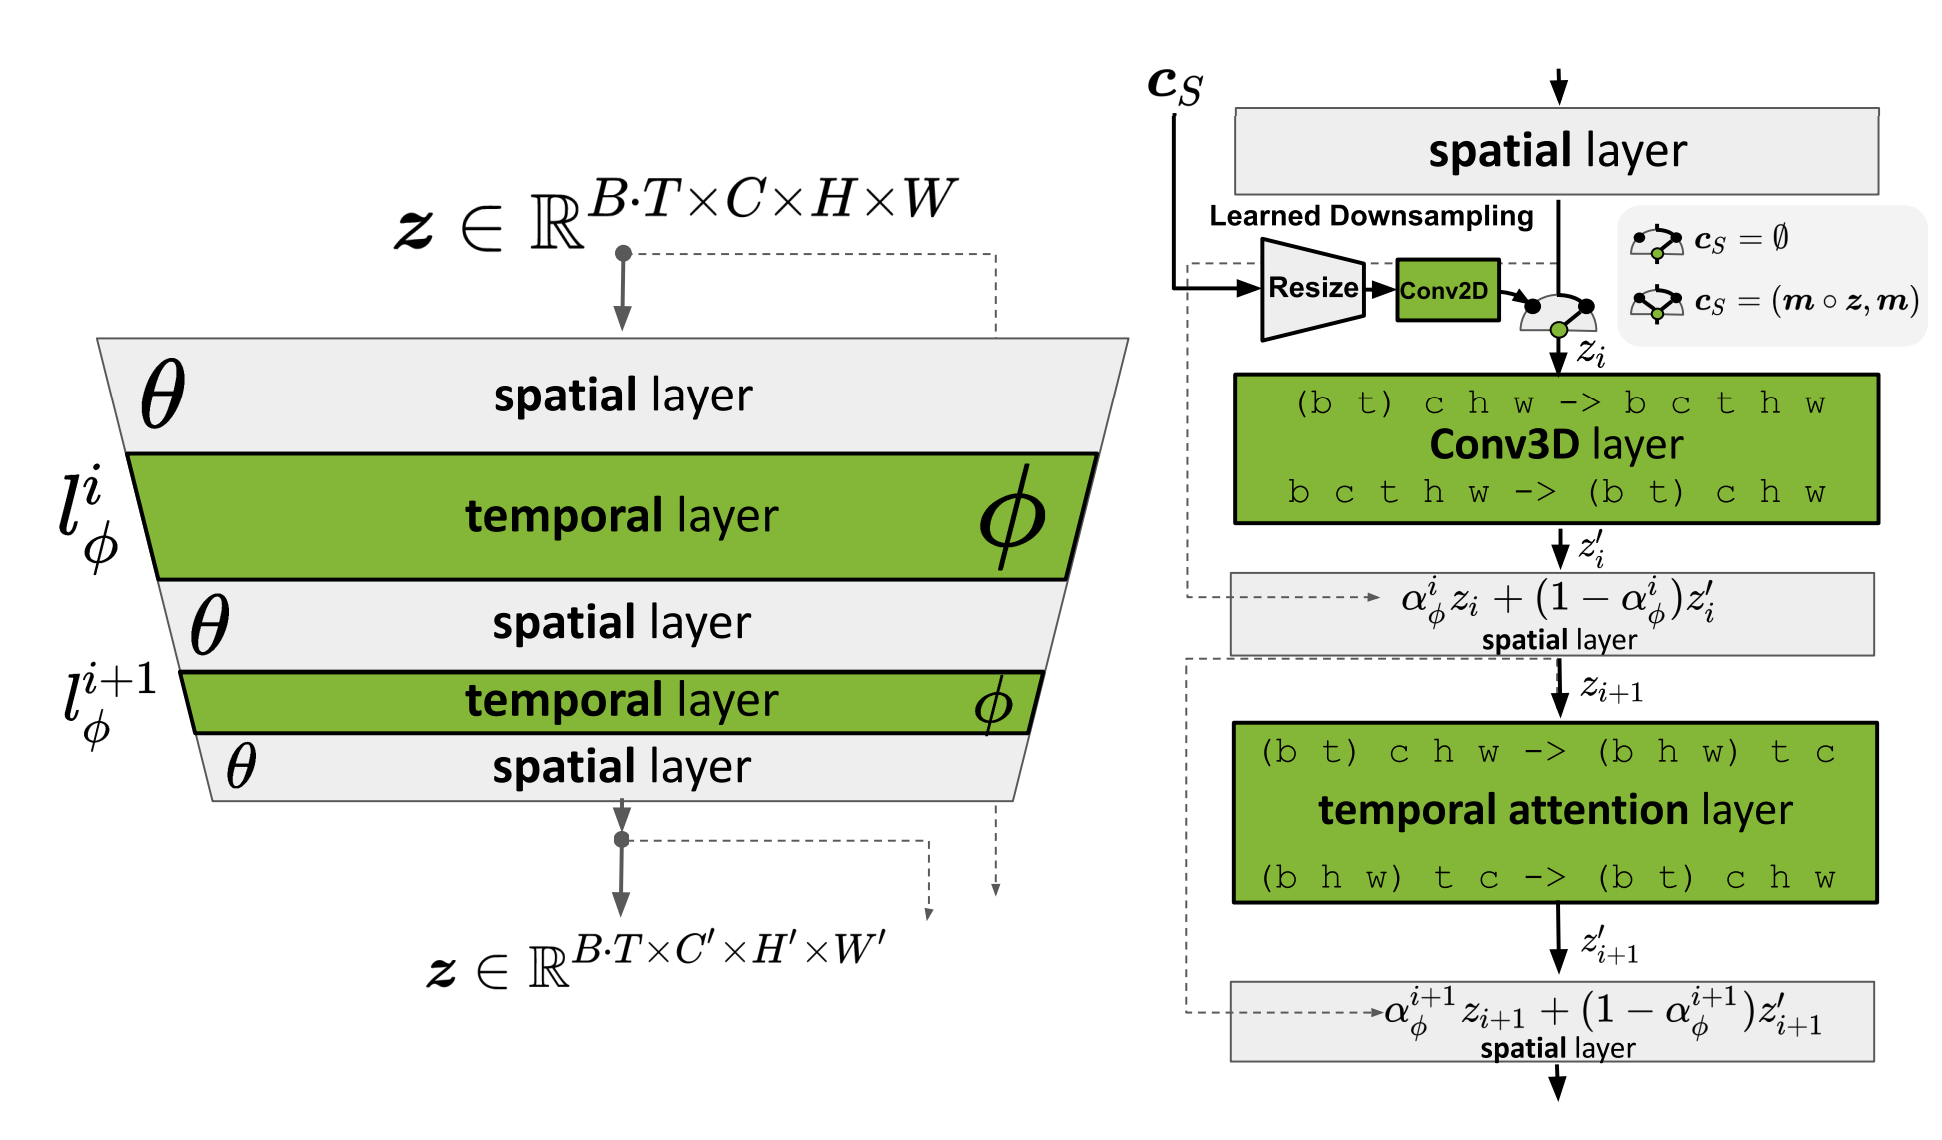
\includegraphics[width=0.6\textwidth]{images/video_ldm/temporal_layers.png}
    \caption{\textit{Left:} The researchers turn pre-trained LDM into video generator by adding temporal layers $l_\phi$ that learn to align images in a temporally consistent manner. The spatial layers $l_\theta$ are frozen and only the temporal layers are learned. \textit{Right:} closer look into spatial, temporal layers of the left side (a single U-Net block). In order to deal with the addition of the temporal dimension, they rearranged the batch dimension in LDM to be mixed with the temporal dimension for the next layer: $(b\ t)\ c\ h\ w \rightarrow b\ t\ c\ h\ w$.}
    \label{fig:video_ldm_spatial_temporal_mixing_layers}
\end{figure}

The architecture of Video-LDM is similar to Stable Diffusion with the exception of added temporal layers.

The input of the spatial layers $l_\theta^i$ is of the dimension $b c h w$ whereas the input dimension of temporal layers is of the dimension $b\ t\ c\ h\ w$. This notation is called \texttt{Einops} and is discussed in the Einops paper \cite{einops}. The spatial layers interpret the video as a batch of images by shifting the temporal axis into the batch dimension (the spatial layers treat all $B \cdot T$ encoded video frames in the batch dimension $b$). And for temporal layers, they reshape the input back to video dimensions using einops (they process entire videos in new temporal dimension $t$): $(b\ t)\ c\ h\ w \rightarrow b\ c\ t\ h\ w$

\textbf{Mixing factor:} after each temporal layer, the output $z'$ is combined with the output of previous spatial layer output $z$ to form a mixing: 

\[\alpha_\phi^i z_{i} + (1 - \alpha_\phi^i) z_{i}'\] 

where $\alpha_\phi^i \in [0, 1]$ and is a learnable parameter. If we set $\alpha = 1$ for each layer we retain native image generation capability, by skipping the temporal blocks. This mixing operation is similar to Classifier-free Guidance (CFG) (mixing between conditional score and unconditional score).

\textbf{Temporal mixing layers:} two types of temporal mixing layers are used (see figure \ref{fig:video_ldm_spatial_temporal_mixing_layers}): \textbf{temporal attention} and \textbf{residual blocks based on 3D convolutions}. The temporal attention layer is similar to the spatial attention layer, but it operates on the temporal dimension.

\textbf{Noise scheduler:} Video-LDM uses the same noise scheduler as the underlying image model. In table 6 of the paper, it shows that in all of their models, they use linear noise scheduler.

\textbf{Training objective:} the training objective is likelihood based, like the LDM objective (score matching objective of predicted niose in U-Net):

\[ \arg \min_\phi \mathbb{E}_{x \sim p_{\text{data}}, \tau \sim p_{\tau}, \epsilon \sim \mathcal{N} (0, I)} \left[ \left| \left| y - f_{\theta,\phi} (z_{\tau} ; c, \tau) \right| \right|^2_2 \right] \]

where $\tau$ is the diffusion time step, $y$ is the target noise vector. The target is to minimize the difference between predicted noise and ground truth $y$ over all video frames (with mean squared error).

\textbf{Adding temporal layers to the autoencoder's decoder:} the researchers add temporal layers to the decoder of the autoencoder which they found this step to be critical for achieving good results. The reason is that the autoencoder is trained on images and flickering artifacts are present in the generated videos. So the researchers fine-tune the decoder on video data with a \textbf{patch-wise temporal discriminator built from 3D convolutions}. The encoder, however, remains unchanged.

\textbf{Temporal binary mask:} generating latents and turning them into video (frame-by-frame prediction - temporal autoregressive) is efficient, but it reaches its limits when generating long duration videos. In order to adapt to longer duration videos, the researchers turned the model as \textit{prediction models} where for each two keyframes, we interpolate between them (divide and conquer). By using binary masks $m_S$ (0 or 1) it indicates the model which frames and the context ($m = 1$) and which frames are to be predicted $m = 0$. The frames are multiplied by the mask and the model learns to predict the missing frames.

\textbf{Higher frame rate:} to achieve high frame rate (high temporal resolution), they predict three interpolated frames between each two keyframes; they call this $T \rightarrow 4T$ interpolation model. Its possible to achieve higher frame rates; its also possible to train $4T \rightarrow 16T$ interpolation model.

\textbf{DDIM Sampling:} in appendix F of the paper they write that they use the sampler from denoising diffusion implicit models (DDIM) \cite{ddim} (section \ref{subsec:ddim_sampler}), where the stochastically $\eta$ is varied, as well as the guidance scale.

